\documentclass[twoside]{book}

% Packages required by doxygen
\usepackage{fixltx2e}
\usepackage{calc}
\usepackage{doxygen}
\usepackage{graphicx}
\usepackage[utf8]{inputenc}
\usepackage{makeidx}
\usepackage{multicol}
\usepackage{multirow}
\PassOptionsToPackage{warn}{textcomp}
\usepackage{textcomp}
\usepackage[nointegrals]{wasysym}
\usepackage[table]{xcolor}

% Font selection
\usepackage[T1]{fontenc}
\usepackage{mathptmx}
\usepackage[scaled=.90]{helvet}
\usepackage{courier}
\usepackage{amssymb}
\usepackage{sectsty}
\renewcommand{\familydefault}{\sfdefault}
\allsectionsfont{%
  \fontseries{bc}\selectfont%
  \color{darkgray}%
}
\renewcommand{\DoxyLabelFont}{%
  \fontseries{bc}\selectfont%
  \color{darkgray}%
}
\newcommand{\+}{\discretionary{\mbox{\scriptsize$\hookleftarrow$}}{}{}}

% Page & text layout
\usepackage{geometry}
\geometry{%
  a4paper,%
  top=2.5cm,%
  bottom=2.5cm,%
  left=2.5cm,%
  right=2.5cm%
}
\tolerance=750
\hfuzz=15pt
\hbadness=750
\setlength{\emergencystretch}{15pt}
\setlength{\parindent}{0cm}
\setlength{\parskip}{0.2cm}
\makeatletter
\renewcommand{\paragraph}{%
  \@startsection{paragraph}{4}{0ex}{-1.0ex}{1.0ex}{%
    \normalfont\normalsize\bfseries\SS@parafont%
  }%
}
\renewcommand{\subparagraph}{%
  \@startsection{subparagraph}{5}{0ex}{-1.0ex}{1.0ex}{%
    \normalfont\normalsize\bfseries\SS@subparafont%
  }%
}
\makeatother

% Headers & footers
\usepackage{fancyhdr}
\pagestyle{fancyplain}
\fancyhead[LE]{\fancyplain{}{\bfseries\thepage}}
\fancyhead[CE]{\fancyplain{}{}}
\fancyhead[RE]{\fancyplain{}{\bfseries\leftmark}}
\fancyhead[LO]{\fancyplain{}{\bfseries\rightmark}}
\fancyhead[CO]{\fancyplain{}{}}
\fancyhead[RO]{\fancyplain{}{\bfseries\thepage}}
\fancyfoot[LE]{\fancyplain{}{}}
\fancyfoot[CE]{\fancyplain{}{}}
\fancyfoot[RE]{\fancyplain{}{\bfseries\scriptsize Generated on Sat Oct 25 2014 00\+:26\+:52 for S\+W\+E1\+D by Doxygen }}
\fancyfoot[LO]{\fancyplain{}{\bfseries\scriptsize Generated on Sat Oct 25 2014 00\+:26\+:52 for S\+W\+E1\+D by Doxygen }}
\fancyfoot[CO]{\fancyplain{}{}}
\fancyfoot[RO]{\fancyplain{}{}}
\renewcommand{\footrulewidth}{0.4pt}
\renewcommand{\chaptermark}[1]{%
  \markboth{#1}{}%
}
\renewcommand{\sectionmark}[1]{%
  \markright{\thesection\ #1}%
}

% Indices & bibliography
\usepackage{natbib}
\usepackage[titles]{tocloft}
\setcounter{tocdepth}{3}
\setcounter{secnumdepth}{5}
\makeindex

% Hyperlinks (required, but should be loaded last)
\usepackage{ifpdf}
\ifpdf
  \usepackage[pdftex,pagebackref=true]{hyperref}
\else
  \usepackage[ps2pdf,pagebackref=true]{hyperref}
\fi
\hypersetup{%
  colorlinks=true,%
  linkcolor=blue,%
  citecolor=blue,%
  unicode%
}

% Custom commands
\newcommand{\clearemptydoublepage}{%
  \newpage{\pagestyle{empty}\cleardoublepage}%
}


%===== C O N T E N T S =====

\begin{document}

% Titlepage & ToC
\hypersetup{pageanchor=false,
             bookmarks=true,
             bookmarksnumbered=true,
             pdfencoding=unicode
            }
\pagenumbering{roman}
\begin{titlepage}
\vspace*{7cm}
\begin{center}%
{\Large S\+W\+E1\+D }\\
\vspace*{1cm}
{\large Generated by Doxygen 1.8.8}\\
\vspace*{0.5cm}
{\small Sat Oct 25 2014 00:26:52}\\
\end{center}
\end{titlepage}
\clearemptydoublepage
\tableofcontents
\clearemptydoublepage
\pagenumbering{arabic}
\hypersetup{pageanchor=true}

%--- Begin generated contents ---
\chapter{Namespace Index}
\section{Namespace List}
Here is a list of all namespaces with brief descriptions\+:\begin{DoxyCompactList}
\item\contentsline{section}{\hyperlink{namespacescenarios}{scenarios} }{\pageref{namespacescenarios}}{}
\item\contentsline{section}{\hyperlink{namespacesolver}{solver} }{\pageref{namespacesolver}}{}
\end{DoxyCompactList}

\chapter{Hierarchical Index}
\section{Class Hierarchy}
This inheritance list is sorted roughly, but not completely, alphabetically\+:\begin{DoxyCompactList}
\item \contentsline{section}{scenarios\+:\+:Dam\+Break}{\pageref{classscenarios_1_1DamBreak}}{}
\item \contentsline{section}{solver\+:\+:F\+Wave$<$ T $>$}{\pageref{classsolver_1_1FWave}}{}
\item \contentsline{section}{solver\+:\+:F\+Wave$<$ T $>$\+:\+:Quantity}{\pageref{structsolver_1_1FWave_1_1Quantity}}{}
\item \contentsline{section}{scenarios\+:\+:Rare\+Rare}{\pageref{classscenarios_1_1RareRare}}{}
\item \contentsline{section}{scenarios\+:\+:Shock\+Shock}{\pageref{classscenarios_1_1ShockShock}}{}
\item Test\+Suite\begin{DoxyCompactList}
\item \contentsline{section}{F\+Wave\+Test}{\pageref{classFWaveTest}}{}
\end{DoxyCompactList}
\end{DoxyCompactList}

\chapter{Class Index}
\section{Class List}
Here are the classes, structs, unions and interfaces with brief descriptions\+:\begin{DoxyCompactList}
\item\contentsline{section}{\hyperlink{classsolver_1_1FWave}{solver\+::\+F\+Wave$<$ T $>$} }{\pageref{classsolver_1_1FWave}}{}
\item\contentsline{section}{\hyperlink{classFWaveTest}{F\+Wave\+Test} }{\pageref{classFWaveTest}}{}
\item\contentsline{section}{\hyperlink{structsolver_1_1FWave_1_1Quantity}{solver\+::\+F\+Wave$<$ T $>$\+::\+Quantity} }{\pageref{structsolver_1_1FWave_1_1Quantity}}{}
\end{DoxyCompactList}

\chapter{File Index}
\section{File List}
Here is a list of all files with brief descriptions\+:\begin{DoxyCompactList}
\item\contentsline{section}{\hyperlink{FWave_8hpp}{F\+Wave.\+hpp} }{\pageref{FWave_8hpp}}{}
\item\contentsline{section}{\hyperlink{FWaveTest_8h}{F\+Wave\+Test.\+h} }{\pageref{FWaveTest_8h}}{}
\item\contentsline{section}{\hyperlink{runncer_8cpp}{runncer.\+cpp} }{\pageref{runncer_8cpp}}{}
\item\contentsline{section}{\hyperlink{runner_8cpp}{runner.\+cpp} }{\pageref{runner_8cpp}}{}
\end{DoxyCompactList}

\chapter{Namespace Documentation}
\hypertarget{namespacesolver}{}\section{solver Namespace Reference}
\label{namespacesolver}\index{solver@{solver}}
\subsection*{Classes}
\begin{DoxyCompactItemize}
\item 
class \hyperlink{classsolver_1_1FWave}{F\+Wave}
\end{DoxyCompactItemize}

\chapter{Class Documentation}
\hypertarget{classsolver_1_1FWave}{}\section{solver\+:\+:F\+Wave$<$ T $>$ Class Template Reference}
\label{classsolver_1_1FWave}\index{solver\+::\+F\+Wave$<$ T $>$@{solver\+::\+F\+Wave$<$ T $>$}}


{\ttfamily \#include $<$F\+Wave.\+hpp$>$}

\subsection*{Classes}
\begin{DoxyCompactItemize}
\item 
struct \hyperlink{structsolver_1_1FWave_1_1Quantity}{Quantity}
\end{DoxyCompactItemize}
\subsection*{Public Member Functions}
\begin{DoxyCompactItemize}
\item 
\hyperlink{classsolver_1_1FWave_a446e2721d799afa5612a3a2b8c30d668}{F\+Wave} ()
\item 
void \hyperlink{classsolver_1_1FWave_a2e7f623f6dc6bd74f49af17dccafd7c7}{compute\+Net\+Updates} (const T \&hl, const T \&hr, const T \&hul, const T \&hur, const T \&bl, const T \&br, T \&outhl, T \&outhr, T \&outhul, T \&outhur, T \&outmax\+W\+S)
\end{DoxyCompactItemize}
\subsection*{Static Public Attributes}
\begin{DoxyCompactItemize}
\item 
static const T \hyperlink{classsolver_1_1FWave_ac3884c16c1822530961884e9f52304a2}{g} = 9.\+81f
\end{DoxyCompactItemize}


\subsection{Constructor \& Destructor Documentation}
\hypertarget{classsolver_1_1FWave_a446e2721d799afa5612a3a2b8c30d668}{}\index{solver\+::\+F\+Wave@{solver\+::\+F\+Wave}!F\+Wave@{F\+Wave}}
\index{F\+Wave@{F\+Wave}!solver\+::\+F\+Wave@{solver\+::\+F\+Wave}}
\subsubsection[{F\+Wave}]{\setlength{\rightskip}{0pt plus 5cm}template$<$typename T$>$ {\bf solver\+::\+F\+Wave}$<$ T $>$\+::{\bf F\+Wave} (
\begin{DoxyParamCaption}
{}
\end{DoxyParamCaption}
)\hspace{0.3cm}{\ttfamily [inline]}}\label{classsolver_1_1FWave_a446e2721d799afa5612a3a2b8c30d668}


\subsection{Member Function Documentation}
\hypertarget{classsolver_1_1FWave_a2e7f623f6dc6bd74f49af17dccafd7c7}{}\index{solver\+::\+F\+Wave@{solver\+::\+F\+Wave}!compute\+Net\+Updates@{compute\+Net\+Updates}}
\index{compute\+Net\+Updates@{compute\+Net\+Updates}!solver\+::\+F\+Wave@{solver\+::\+F\+Wave}}
\subsubsection[{compute\+Net\+Updates}]{\setlength{\rightskip}{0pt plus 5cm}template$<$typename T$>$ void {\bf solver\+::\+F\+Wave}$<$ T $>$\+::compute\+Net\+Updates (
\begin{DoxyParamCaption}
\item[{const T \&}]{hl, }
\item[{const T \&}]{hr, }
\item[{const T \&}]{hul, }
\item[{const T \&}]{hur, }
\item[{const T \&}]{bl, }
\item[{const T \&}]{br, }
\item[{T \&}]{outhl, }
\item[{T \&}]{outhr, }
\item[{T \&}]{outhul, }
\item[{T \&}]{outhur, }
\item[{T \&}]{outmax\+W\+S}
\end{DoxyParamCaption}
)\hspace{0.3cm}{\ttfamily [inline]}}\label{classsolver_1_1FWave_a2e7f623f6dc6bd74f49af17dccafd7c7}
Compute left and right going net-\/updates.


\begin{DoxyParams}{Parameters}
{\em \&hl} & height on the left side of the edge. \\
\hline
{\em \&hr} & height on the right side of the edge. \\
\hline
{\em \&hul} & momentum on the left side of the edge. \\
\hline
{\em \&hur} & momentum on the right side of the edge. \\
\hline
{\em \&bl} & bathymetry on the left side of the edge. \\
\hline
{\em \&br} & bathymetry on the right side of the edge.\\
\hline
{\em \&outhl} & output height of the cell on the left side of the edge. \\
\hline
{\em \&outhr} & output height of the cell on the right side of the edge. \\
\hline
{\em \&outhul} & output momentum of the cell on the left side of the edge. \\
\hline
{\em \&outhur} & output momentum of the cell on the right side of the edge. \\
\hline
{\em \&outmax\+W\+S} & will be set to\+: Maximum (linearized) wave speed -\/$>$ Should be used in the C\+F\+L-\/condition. \\
\hline
\end{DoxyParams}


\subsection{Member Data Documentation}
\hypertarget{classsolver_1_1FWave_ac3884c16c1822530961884e9f52304a2}{}\index{solver\+::\+F\+Wave@{solver\+::\+F\+Wave}!g@{g}}
\index{g@{g}!solver\+::\+F\+Wave@{solver\+::\+F\+Wave}}
\subsubsection[{g}]{\setlength{\rightskip}{0pt plus 5cm}template$<$typename T$>$ const T {\bf solver\+::\+F\+Wave}$<$ T $>$\+::g = 9.\+81f\hspace{0.3cm}{\ttfamily [static]}}\label{classsolver_1_1FWave_ac3884c16c1822530961884e9f52304a2}


The documentation for this class was generated from the following file\+:\begin{DoxyCompactItemize}
\item 
\hyperlink{FWave_8hpp}{F\+Wave.\+hpp}\end{DoxyCompactItemize}

\hypertarget{classFWaveTest}{}\section{F\+Wave\+Test Class Reference}
\label{classFWaveTest}\index{F\+Wave\+Test@{F\+Wave\+Test}}


{\ttfamily \#include $<$F\+Wave\+Test.\+h$>$}

Inheritance diagram for F\+Wave\+Test\+:\begin{figure}[H]
\begin{center}
\leavevmode
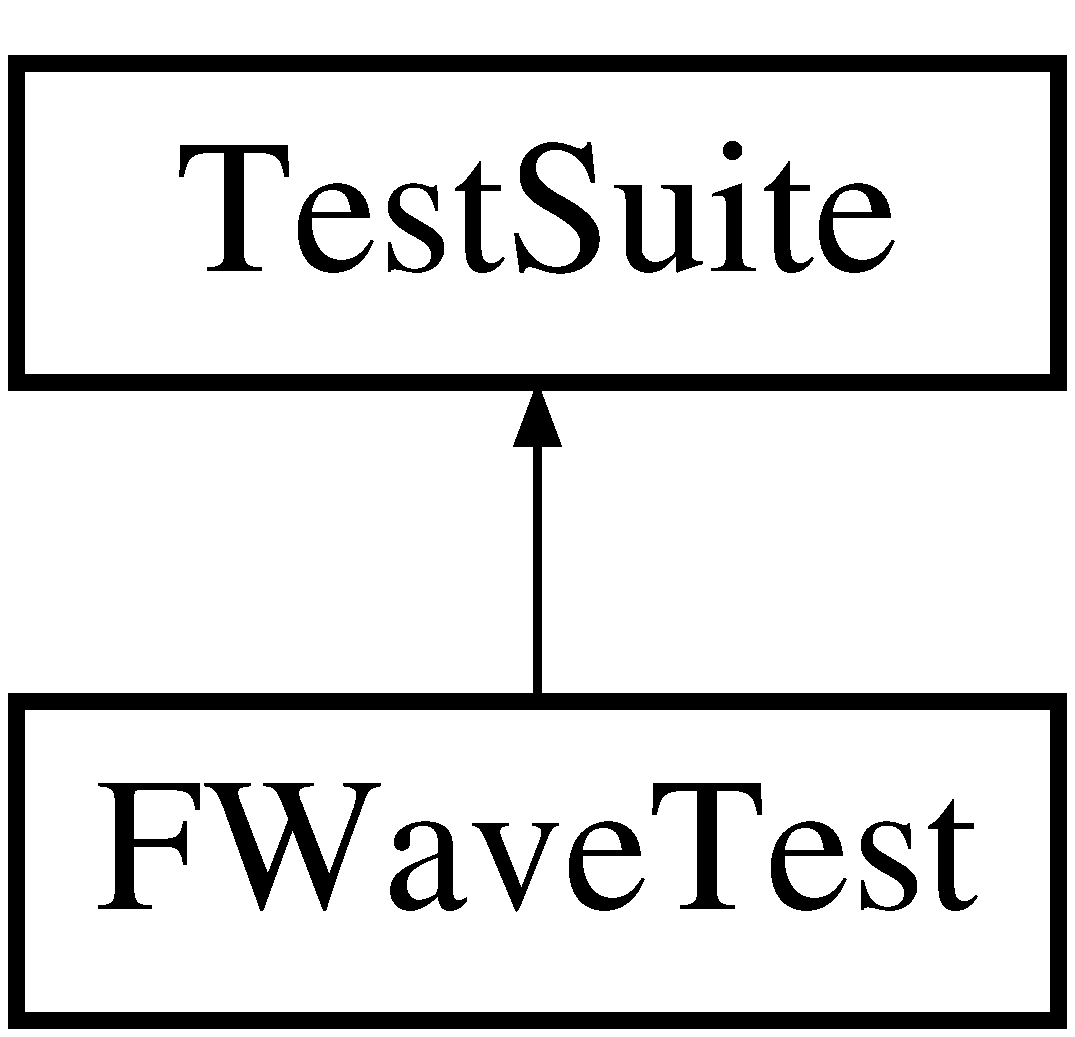
\includegraphics[height=2.000000cm]{classFWaveTest}
\end{center}
\end{figure}
\subsection*{Public Member Functions}
\begin{DoxyCompactItemize}
\item 
\hyperlink{classFWaveTest_a637e3a21850ed7432394b19d1f8320d1}{F\+Wave\+Test} ()
\item 
void \hyperlink{classFWaveTest_aad1779e385672a5fcea0fb09cbd8a2f0}{test\+Same\+Height\+No\+Speed} (void)
\item 
void \hyperlink{classFWaveTest_aed2db9d70b98e7b7924fcb8705bbf509}{test\+Same\+Height\+Left\+Speed} (void)
\item 
void \hyperlink{classFWaveTest_a4cffba9a84aeb963b6b8d4ac79efe227}{test\+Same\+Height\+Right\+Speed} (void)
\item 
void \hyperlink{classFWaveTest_a284fbedaff0f4e2a98ec868926176773}{test\+Same\+Height\+Left\+Right\+Speed} (void)
\item 
void \hyperlink{classFWaveTest_a5ceb6cf106458f0a0110ac13fe2c3f35}{test\+Same\+Height\+Right\+Left\+Speed} (void)
\item 
void \hyperlink{classFWaveTest_abf28f88dc07c66d8ccd7541a2fc9b901}{test\+Decreasing\+Height\+No\+Speed} (void)
\item 
void \hyperlink{classFWaveTest_a817892593d58cf1dad61a2abb0810378}{test\+Decreasing\+Height\+Left\+Speed} (void)
\item 
void \hyperlink{classFWaveTest_aaae1f57e2ef62d53bff1169d84aa7059}{test\+Decreasing\+Height\+Right\+Speed} (void)
\item 
void \hyperlink{classFWaveTest_a2dc496f15de60f5d199d6b1a35b596f3}{test\+Decreasing\+Height\+Left\+Right\+Speed} (void)
\item 
void \hyperlink{classFWaveTest_a24b35d3400c5ee91be94bf7ba47e82bf}{test\+Decreasing\+Height\+Right\+Left\+Speed} (void)
\item 
void \hyperlink{classFWaveTest_abd75e73da77f86f5145dd9ed1796f0fc}{test\+Increasing\+Height\+No\+Speed} (void)
\item 
void \hyperlink{classFWaveTest_aa6a036225ee4f6a00d40ba439899933d}{test\+Increasing\+Height\+Left\+Speed} (void)
\item 
void \hyperlink{classFWaveTest_a3e4e03f910ee006e0dce95cb2276a76a}{test\+Increasing\+Height\+Right\+Speed} (void)
\item 
void \hyperlink{classFWaveTest_a57b9d687f5a7311739883c9931d1e301}{test\+Increasing\+Height\+Left\+Right\+Speed} (void)
\item 
void \hyperlink{classFWaveTest_aaf371e755b499555a6daf142c9e5173f}{test\+Increasing\+Height\+Right\+Left\+Speed} (void)
\end{DoxyCompactItemize}
\subsection*{Public Attributes}
\begin{DoxyCompactItemize}
\item 
\hyperlink{classsolver_1_1FWave}{solver\+::\+F\+Wave}$<$ T $>$ \hyperlink{classFWaveTest_a195e044738f434127bedf96c2153f230}{fwave}
\end{DoxyCompactItemize}
\subsection*{Static Public Attributes}
\begin{DoxyCompactItemize}
\item 
static const T \hyperlink{classFWaveTest_a8a0b6ebec0c270760dde9af243fc9045}{delta} = 0.\+0001f
\end{DoxyCompactItemize}


\subsection{Constructor \& Destructor Documentation}
\hypertarget{classFWaveTest_a637e3a21850ed7432394b19d1f8320d1}{}\index{F\+Wave\+Test@{F\+Wave\+Test}!F\+Wave\+Test@{F\+Wave\+Test}}
\index{F\+Wave\+Test@{F\+Wave\+Test}!F\+Wave\+Test@{F\+Wave\+Test}}
\subsubsection[{F\+Wave\+Test}]{\setlength{\rightskip}{0pt plus 5cm}F\+Wave\+Test\+::\+F\+Wave\+Test (
\begin{DoxyParamCaption}
{}
\end{DoxyParamCaption}
)\hspace{0.3cm}{\ttfamily [inline]}}\label{classFWaveTest_a637e3a21850ed7432394b19d1f8320d1}


\subsection{Member Function Documentation}
\hypertarget{classFWaveTest_a2dc496f15de60f5d199d6b1a35b596f3}{}\index{F\+Wave\+Test@{F\+Wave\+Test}!test\+Decreasing\+Height\+Left\+Right\+Speed@{test\+Decreasing\+Height\+Left\+Right\+Speed}}
\index{test\+Decreasing\+Height\+Left\+Right\+Speed@{test\+Decreasing\+Height\+Left\+Right\+Speed}!F\+Wave\+Test@{F\+Wave\+Test}}
\subsubsection[{test\+Decreasing\+Height\+Left\+Right\+Speed}]{\setlength{\rightskip}{0pt plus 5cm}void F\+Wave\+Test\+::test\+Decreasing\+Height\+Left\+Right\+Speed (
\begin{DoxyParamCaption}
\item[{void}]{}
\end{DoxyParamCaption}
)\hspace{0.3cm}{\ttfamily [inline]}}\label{classFWaveTest_a2dc496f15de60f5d199d6b1a35b596f3}
Tests F\+Wave\+::compute\+Net\+Updates with the following parameters\+:~\newline
 hl = 10.\+0~\newline
 hr = 5.\+0~\newline
 ~\newline
 hul = -\/2.\+0~\newline
 hur = 3.\+0~\newline
 ~\newline
 bl = 0~\newline
 br = 0~\newline
 \hypertarget{classFWaveTest_a817892593d58cf1dad61a2abb0810378}{}\index{F\+Wave\+Test@{F\+Wave\+Test}!test\+Decreasing\+Height\+Left\+Speed@{test\+Decreasing\+Height\+Left\+Speed}}
\index{test\+Decreasing\+Height\+Left\+Speed@{test\+Decreasing\+Height\+Left\+Speed}!F\+Wave\+Test@{F\+Wave\+Test}}
\subsubsection[{test\+Decreasing\+Height\+Left\+Speed}]{\setlength{\rightskip}{0pt plus 5cm}void F\+Wave\+Test\+::test\+Decreasing\+Height\+Left\+Speed (
\begin{DoxyParamCaption}
\item[{void}]{}
\end{DoxyParamCaption}
)\hspace{0.3cm}{\ttfamily [inline]}}\label{classFWaveTest_a817892593d58cf1dad61a2abb0810378}
Tests F\+Wave\+::compute\+Net\+Updates with the following parameters\+:~\newline
 hl = 10.\+0~\newline
 hr = 5.\+0~\newline
 ~\newline
 hul = -\/2.\+0~\newline
 hur = -\/3.\+0~\newline
 ~\newline
 bl = 0~\newline
 br = 0~\newline
 \hypertarget{classFWaveTest_abf28f88dc07c66d8ccd7541a2fc9b901}{}\index{F\+Wave\+Test@{F\+Wave\+Test}!test\+Decreasing\+Height\+No\+Speed@{test\+Decreasing\+Height\+No\+Speed}}
\index{test\+Decreasing\+Height\+No\+Speed@{test\+Decreasing\+Height\+No\+Speed}!F\+Wave\+Test@{F\+Wave\+Test}}
\subsubsection[{test\+Decreasing\+Height\+No\+Speed}]{\setlength{\rightskip}{0pt plus 5cm}void F\+Wave\+Test\+::test\+Decreasing\+Height\+No\+Speed (
\begin{DoxyParamCaption}
\item[{void}]{}
\end{DoxyParamCaption}
)\hspace{0.3cm}{\ttfamily [inline]}}\label{classFWaveTest_abf28f88dc07c66d8ccd7541a2fc9b901}
Tests F\+Wave\+::compute\+Net\+Updates with the following parameters\+:~\newline
 hl = 10.\+0~\newline
 hr = 5.\+0~\newline
 ~\newline
 hul = 0~\newline
 hur = 0~\newline
 ~\newline
 bl = 0~\newline
 br = 0~\newline
 \hypertarget{classFWaveTest_a24b35d3400c5ee91be94bf7ba47e82bf}{}\index{F\+Wave\+Test@{F\+Wave\+Test}!test\+Decreasing\+Height\+Right\+Left\+Speed@{test\+Decreasing\+Height\+Right\+Left\+Speed}}
\index{test\+Decreasing\+Height\+Right\+Left\+Speed@{test\+Decreasing\+Height\+Right\+Left\+Speed}!F\+Wave\+Test@{F\+Wave\+Test}}
\subsubsection[{test\+Decreasing\+Height\+Right\+Left\+Speed}]{\setlength{\rightskip}{0pt plus 5cm}void F\+Wave\+Test\+::test\+Decreasing\+Height\+Right\+Left\+Speed (
\begin{DoxyParamCaption}
\item[{void}]{}
\end{DoxyParamCaption}
)\hspace{0.3cm}{\ttfamily [inline]}}\label{classFWaveTest_a24b35d3400c5ee91be94bf7ba47e82bf}
Tests F\+Wave\+::compute\+Net\+Updates with the following parameters\+:~\newline
 hl = 10.\+0~\newline
 hr = 5.\+0~\newline
 ~\newline
 hul = 3.\+0~\newline
 hur = -\/2.\+0~\newline
 ~\newline
 bl = 0~\newline
 br = 0~\newline
 \hypertarget{classFWaveTest_aaae1f57e2ef62d53bff1169d84aa7059}{}\index{F\+Wave\+Test@{F\+Wave\+Test}!test\+Decreasing\+Height\+Right\+Speed@{test\+Decreasing\+Height\+Right\+Speed}}
\index{test\+Decreasing\+Height\+Right\+Speed@{test\+Decreasing\+Height\+Right\+Speed}!F\+Wave\+Test@{F\+Wave\+Test}}
\subsubsection[{test\+Decreasing\+Height\+Right\+Speed}]{\setlength{\rightskip}{0pt plus 5cm}void F\+Wave\+Test\+::test\+Decreasing\+Height\+Right\+Speed (
\begin{DoxyParamCaption}
\item[{void}]{}
\end{DoxyParamCaption}
)\hspace{0.3cm}{\ttfamily [inline]}}\label{classFWaveTest_aaae1f57e2ef62d53bff1169d84aa7059}
Tests F\+Wave\+::compute\+Net\+Updates with the following parameters\+:~\newline
 hl = 10.\+0~\newline
 hr = 5.\+0~\newline
 ~\newline
 hul = 3.\+0~\newline
 hur = 2.\+0~\newline
 ~\newline
 bl = 0~\newline
 br = 0~\newline
 \hypertarget{classFWaveTest_a57b9d687f5a7311739883c9931d1e301}{}\index{F\+Wave\+Test@{F\+Wave\+Test}!test\+Increasing\+Height\+Left\+Right\+Speed@{test\+Increasing\+Height\+Left\+Right\+Speed}}
\index{test\+Increasing\+Height\+Left\+Right\+Speed@{test\+Increasing\+Height\+Left\+Right\+Speed}!F\+Wave\+Test@{F\+Wave\+Test}}
\subsubsection[{test\+Increasing\+Height\+Left\+Right\+Speed}]{\setlength{\rightskip}{0pt plus 5cm}void F\+Wave\+Test\+::test\+Increasing\+Height\+Left\+Right\+Speed (
\begin{DoxyParamCaption}
\item[{void}]{}
\end{DoxyParamCaption}
)\hspace{0.3cm}{\ttfamily [inline]}}\label{classFWaveTest_a57b9d687f5a7311739883c9931d1e301}
Tests F\+Wave\+::compute\+Net\+Updates with the following parameters\+:~\newline
 hl = 5.\+0~\newline
 hr = 10.\+0~\newline
 ~\newline
 hul = -\/3.\+0~\newline
 hur = 2.\+0~\newline
 ~\newline
 bl = 0~\newline
 br = 0~\newline
 \hypertarget{classFWaveTest_aa6a036225ee4f6a00d40ba439899933d}{}\index{F\+Wave\+Test@{F\+Wave\+Test}!test\+Increasing\+Height\+Left\+Speed@{test\+Increasing\+Height\+Left\+Speed}}
\index{test\+Increasing\+Height\+Left\+Speed@{test\+Increasing\+Height\+Left\+Speed}!F\+Wave\+Test@{F\+Wave\+Test}}
\subsubsection[{test\+Increasing\+Height\+Left\+Speed}]{\setlength{\rightskip}{0pt plus 5cm}void F\+Wave\+Test\+::test\+Increasing\+Height\+Left\+Speed (
\begin{DoxyParamCaption}
\item[{void}]{}
\end{DoxyParamCaption}
)\hspace{0.3cm}{\ttfamily [inline]}}\label{classFWaveTest_aa6a036225ee4f6a00d40ba439899933d}
Tests F\+Wave\+::compute\+Net\+Updates with the following parameters\+:~\newline
 hl = 5.\+0~\newline
 hr = 10.\+0~\newline
 ~\newline
 hul = -\/3.\+0~\newline
 hur = -\/2.\+0~\newline
 ~\newline
 bl = 0~\newline
 br = 0~\newline
 \hypertarget{classFWaveTest_abd75e73da77f86f5145dd9ed1796f0fc}{}\index{F\+Wave\+Test@{F\+Wave\+Test}!test\+Increasing\+Height\+No\+Speed@{test\+Increasing\+Height\+No\+Speed}}
\index{test\+Increasing\+Height\+No\+Speed@{test\+Increasing\+Height\+No\+Speed}!F\+Wave\+Test@{F\+Wave\+Test}}
\subsubsection[{test\+Increasing\+Height\+No\+Speed}]{\setlength{\rightskip}{0pt plus 5cm}void F\+Wave\+Test\+::test\+Increasing\+Height\+No\+Speed (
\begin{DoxyParamCaption}
\item[{void}]{}
\end{DoxyParamCaption}
)\hspace{0.3cm}{\ttfamily [inline]}}\label{classFWaveTest_abd75e73da77f86f5145dd9ed1796f0fc}
Tests F\+Wave\+::compute\+Net\+Updates with the following parameters\+:~\newline
 hl = 5.\+0~\newline
 hr = 10.\+0~\newline
 ~\newline
 hul = 0~\newline
 hur = 0~\newline
 ~\newline
 bl = 0~\newline
 br = 0~\newline
 \hypertarget{classFWaveTest_aaf371e755b499555a6daf142c9e5173f}{}\index{F\+Wave\+Test@{F\+Wave\+Test}!test\+Increasing\+Height\+Right\+Left\+Speed@{test\+Increasing\+Height\+Right\+Left\+Speed}}
\index{test\+Increasing\+Height\+Right\+Left\+Speed@{test\+Increasing\+Height\+Right\+Left\+Speed}!F\+Wave\+Test@{F\+Wave\+Test}}
\subsubsection[{test\+Increasing\+Height\+Right\+Left\+Speed}]{\setlength{\rightskip}{0pt plus 5cm}void F\+Wave\+Test\+::test\+Increasing\+Height\+Right\+Left\+Speed (
\begin{DoxyParamCaption}
\item[{void}]{}
\end{DoxyParamCaption}
)\hspace{0.3cm}{\ttfamily [inline]}}\label{classFWaveTest_aaf371e755b499555a6daf142c9e5173f}
Tests F\+Wave\+::compute\+Net\+Updates with the following parameters\+:~\newline
 hl = 5.\+0~\newline
 hr = 10.\+0~\newline
 ~\newline
 hul = 2.\+0~\newline
 hur = -\/3.\+0~\newline
 ~\newline
 bl = 0~\newline
 br = 0~\newline
 \hypertarget{classFWaveTest_a3e4e03f910ee006e0dce95cb2276a76a}{}\index{F\+Wave\+Test@{F\+Wave\+Test}!test\+Increasing\+Height\+Right\+Speed@{test\+Increasing\+Height\+Right\+Speed}}
\index{test\+Increasing\+Height\+Right\+Speed@{test\+Increasing\+Height\+Right\+Speed}!F\+Wave\+Test@{F\+Wave\+Test}}
\subsubsection[{test\+Increasing\+Height\+Right\+Speed}]{\setlength{\rightskip}{0pt plus 5cm}void F\+Wave\+Test\+::test\+Increasing\+Height\+Right\+Speed (
\begin{DoxyParamCaption}
\item[{void}]{}
\end{DoxyParamCaption}
)\hspace{0.3cm}{\ttfamily [inline]}}\label{classFWaveTest_a3e4e03f910ee006e0dce95cb2276a76a}
Tests F\+Wave\+::compute\+Net\+Updates with the following parameters\+:~\newline
 hl = 5.\+0~\newline
 hr = 10.\+0~\newline
 ~\newline
 hul = 2.\+0~\newline
 hur = 3.\+0~\newline
 ~\newline
 bl = 0~\newline
 br = 0~\newline
 \hypertarget{classFWaveTest_a284fbedaff0f4e2a98ec868926176773}{}\index{F\+Wave\+Test@{F\+Wave\+Test}!test\+Same\+Height\+Left\+Right\+Speed@{test\+Same\+Height\+Left\+Right\+Speed}}
\index{test\+Same\+Height\+Left\+Right\+Speed@{test\+Same\+Height\+Left\+Right\+Speed}!F\+Wave\+Test@{F\+Wave\+Test}}
\subsubsection[{test\+Same\+Height\+Left\+Right\+Speed}]{\setlength{\rightskip}{0pt plus 5cm}void F\+Wave\+Test\+::test\+Same\+Height\+Left\+Right\+Speed (
\begin{DoxyParamCaption}
\item[{void}]{}
\end{DoxyParamCaption}
)\hspace{0.3cm}{\ttfamily [inline]}}\label{classFWaveTest_a284fbedaff0f4e2a98ec868926176773}
Tests F\+Wave\+::compute\+Net\+Updates with the following parameters\+:~\newline
 hl = 5.\+0~\newline
 hr = 5.\+0~\newline
 ~\newline
 hul = -\/3.\+0~\newline
 hur = 2.\+0~\newline
 ~\newline
 bl = 0~\newline
 br = 0~\newline
 \hypertarget{classFWaveTest_aed2db9d70b98e7b7924fcb8705bbf509}{}\index{F\+Wave\+Test@{F\+Wave\+Test}!test\+Same\+Height\+Left\+Speed@{test\+Same\+Height\+Left\+Speed}}
\index{test\+Same\+Height\+Left\+Speed@{test\+Same\+Height\+Left\+Speed}!F\+Wave\+Test@{F\+Wave\+Test}}
\subsubsection[{test\+Same\+Height\+Left\+Speed}]{\setlength{\rightskip}{0pt plus 5cm}void F\+Wave\+Test\+::test\+Same\+Height\+Left\+Speed (
\begin{DoxyParamCaption}
\item[{void}]{}
\end{DoxyParamCaption}
)\hspace{0.3cm}{\ttfamily [inline]}}\label{classFWaveTest_aed2db9d70b98e7b7924fcb8705bbf509}
Tests F\+Wave\+::compute\+Net\+Updates with the following parameters\+:~\newline
 hl = 5.\+0~\newline
 hr = 5.\+0~\newline
 ~\newline
 hul = -\/2.\+0~\newline
 hur = -\/3.\+0~\newline
 ~\newline
 bl = 0~\newline
 br = 0~\newline
 \hypertarget{classFWaveTest_aad1779e385672a5fcea0fb09cbd8a2f0}{}\index{F\+Wave\+Test@{F\+Wave\+Test}!test\+Same\+Height\+No\+Speed@{test\+Same\+Height\+No\+Speed}}
\index{test\+Same\+Height\+No\+Speed@{test\+Same\+Height\+No\+Speed}!F\+Wave\+Test@{F\+Wave\+Test}}
\subsubsection[{test\+Same\+Height\+No\+Speed}]{\setlength{\rightskip}{0pt plus 5cm}void F\+Wave\+Test\+::test\+Same\+Height\+No\+Speed (
\begin{DoxyParamCaption}
\item[{void}]{}
\end{DoxyParamCaption}
)\hspace{0.3cm}{\ttfamily [inline]}}\label{classFWaveTest_aad1779e385672a5fcea0fb09cbd8a2f0}
Tests F\+Wave\+::compute\+Net\+Updates with the following parameters\+:~\newline
 hl = 5.\+0~\newline
 hr = 5.\+0~\newline
 ~\newline
 hul = 0~\newline
 hur = 0~\newline
 ~\newline
 bl = 0~\newline
 br = 0~\newline
 \hypertarget{classFWaveTest_a5ceb6cf106458f0a0110ac13fe2c3f35}{}\index{F\+Wave\+Test@{F\+Wave\+Test}!test\+Same\+Height\+Right\+Left\+Speed@{test\+Same\+Height\+Right\+Left\+Speed}}
\index{test\+Same\+Height\+Right\+Left\+Speed@{test\+Same\+Height\+Right\+Left\+Speed}!F\+Wave\+Test@{F\+Wave\+Test}}
\subsubsection[{test\+Same\+Height\+Right\+Left\+Speed}]{\setlength{\rightskip}{0pt plus 5cm}void F\+Wave\+Test\+::test\+Same\+Height\+Right\+Left\+Speed (
\begin{DoxyParamCaption}
\item[{void}]{}
\end{DoxyParamCaption}
)\hspace{0.3cm}{\ttfamily [inline]}}\label{classFWaveTest_a5ceb6cf106458f0a0110ac13fe2c3f35}
Tests F\+Wave\+::compute\+Net\+Updates with the following parameters\+:~\newline
 hl = 5.\+0~\newline
 hr = 5.\+0~\newline
 ~\newline
 hul = 2.\+0~\newline
 hur = -\/3.\+0~\newline
 ~\newline
 bl = 0~\newline
 br = 0~\newline
 \hypertarget{classFWaveTest_a4cffba9a84aeb963b6b8d4ac79efe227}{}\index{F\+Wave\+Test@{F\+Wave\+Test}!test\+Same\+Height\+Right\+Speed@{test\+Same\+Height\+Right\+Speed}}
\index{test\+Same\+Height\+Right\+Speed@{test\+Same\+Height\+Right\+Speed}!F\+Wave\+Test@{F\+Wave\+Test}}
\subsubsection[{test\+Same\+Height\+Right\+Speed}]{\setlength{\rightskip}{0pt plus 5cm}void F\+Wave\+Test\+::test\+Same\+Height\+Right\+Speed (
\begin{DoxyParamCaption}
\item[{void}]{}
\end{DoxyParamCaption}
)\hspace{0.3cm}{\ttfamily [inline]}}\label{classFWaveTest_a4cffba9a84aeb963b6b8d4ac79efe227}
Tests F\+Wave\+::compute\+Net\+Updates with the following parameters\+:~\newline
 hl = 5.\+0~\newline
 hr = 5.\+0~\newline
 ~\newline
 hul = 3.\+0~\newline
 hur = 2.\+0~\newline
 ~\newline
 bl = 0~\newline
 br = 0~\newline
 

\subsection{Member Data Documentation}
\hypertarget{classFWaveTest_a8a0b6ebec0c270760dde9af243fc9045}{}\index{F\+Wave\+Test@{F\+Wave\+Test}!delta@{delta}}
\index{delta@{delta}!F\+Wave\+Test@{F\+Wave\+Test}}
\subsubsection[{delta}]{\setlength{\rightskip}{0pt plus 5cm}const T F\+Wave\+Test\+::delta = 0.\+0001f\hspace{0.3cm}{\ttfamily [static]}}\label{classFWaveTest_a8a0b6ebec0c270760dde9af243fc9045}
Delta used for comparing expected and actual values \hypertarget{classFWaveTest_a195e044738f434127bedf96c2153f230}{}\index{F\+Wave\+Test@{F\+Wave\+Test}!fwave@{fwave}}
\index{fwave@{fwave}!F\+Wave\+Test@{F\+Wave\+Test}}
\subsubsection[{fwave}]{\setlength{\rightskip}{0pt plus 5cm}{\bf solver\+::\+F\+Wave}$<$T$>$ F\+Wave\+Test\+::fwave}\label{classFWaveTest_a195e044738f434127bedf96c2153f230}
F\+Wave to test 

The documentation for this class was generated from the following file\+:\begin{DoxyCompactItemize}
\item 
solvers/\hyperlink{FWaveTest_8h}{F\+Wave\+Test.\+h}\end{DoxyCompactItemize}

\hypertarget{structsolver_1_1FWave_1_1Quantity}{}\section{solver\+:\+:F\+Wave$<$ T $>$\+:\+:Quantity Struct Reference}
\label{structsolver_1_1FWave_1_1Quantity}\index{solver\+::\+F\+Wave$<$ T $>$\+::\+Quantity@{solver\+::\+F\+Wave$<$ T $>$\+::\+Quantity}}


{\ttfamily \#include $<$F\+Wave.\+hpp$>$}

\subsection*{Public Attributes}
\begin{DoxyCompactItemize}
\item 
T \hyperlink{structsolver_1_1FWave_1_1Quantity_ab21e966b42ed55a04b852deb96ec7285}{h}
\item 
T \hyperlink{structsolver_1_1FWave_1_1Quantity_a85b3d7be51ca5dc26a031d421c16095c}{hu}
\end{DoxyCompactItemize}


\subsection{Member Data Documentation}
\hypertarget{structsolver_1_1FWave_1_1Quantity_ab21e966b42ed55a04b852deb96ec7285}{}\index{solver\+::\+F\+Wave\+::\+Quantity@{solver\+::\+F\+Wave\+::\+Quantity}!h@{h}}
\index{h@{h}!solver\+::\+F\+Wave\+::\+Quantity@{solver\+::\+F\+Wave\+::\+Quantity}}
\subsubsection[{h}]{\setlength{\rightskip}{0pt plus 5cm}template$<$typename T$>$ T {\bf solver\+::\+F\+Wave}$<$ T $>$\+::Quantity\+::h}\label{structsolver_1_1FWave_1_1Quantity_ab21e966b42ed55a04b852deb96ec7285}
\hypertarget{structsolver_1_1FWave_1_1Quantity_a85b3d7be51ca5dc26a031d421c16095c}{}\index{solver\+::\+F\+Wave\+::\+Quantity@{solver\+::\+F\+Wave\+::\+Quantity}!hu@{hu}}
\index{hu@{hu}!solver\+::\+F\+Wave\+::\+Quantity@{solver\+::\+F\+Wave\+::\+Quantity}}
\subsubsection[{hu}]{\setlength{\rightskip}{0pt plus 5cm}template$<$typename T$>$ T {\bf solver\+::\+F\+Wave}$<$ T $>$\+::Quantity\+::hu}\label{structsolver_1_1FWave_1_1Quantity_a85b3d7be51ca5dc26a031d421c16095c}


The documentation for this struct was generated from the following file\+:\begin{DoxyCompactItemize}
\item 
solvers/\hyperlink{FWave_8hpp}{F\+Wave.\+hpp}\end{DoxyCompactItemize}

\chapter{File Documentation}
\hypertarget{FWave_8hpp}{}\section{F\+Wave.\+hpp File Reference}
\label{FWave_8hpp}\index{F\+Wave.\+hpp@{F\+Wave.\+hpp}}
{\ttfamily \#include $<$cassert$>$}\\*
{\ttfamily \#include $<$cmath$>$}\\*
{\ttfamily \#include $<$iostream$>$}\\*
\subsection*{Classes}
\begin{DoxyCompactItemize}
\item 
class \hyperlink{classsolver_1_1FWave}{solver\+::\+F\+Wave$<$ T $>$}
\item 
class \hyperlink{classsolver_1_1FWave}{solver\+::\+F\+Wave$<$ T $>$}
\item 
struct \hyperlink{structsolver_1_1FWave_1_1Quantity}{solver\+::\+F\+Wave$<$ T $>$\+::\+Quantity}
\end{DoxyCompactItemize}
\subsection*{Namespaces}
\begin{DoxyCompactItemize}
\item 
 \hyperlink{namespacesolver}{solver}
\end{DoxyCompactItemize}

\hypertarget{FWaveTest_8h}{}\section{solvers/\+F\+Wave\+Test.h File Reference}
\label{FWaveTest_8h}\index{solvers/\+F\+Wave\+Test.\+h@{solvers/\+F\+Wave\+Test.\+h}}
{\ttfamily \#include $<$cxxtest/\+Test\+Suite.\+h$>$}\\*
{\ttfamily \#include \char`\"{}../../\+Tsunami\+Original/\+S\+W\+E1\+D/src/types.\+h\char`\"{}}\\*
{\ttfamily \#include \char`\"{}F\+Wave.\+hpp\char`\"{}}\\*
\subsection*{Classes}
\begin{DoxyCompactItemize}
\item 
class \hyperlink{classFWaveTest}{F\+Wave\+Test}
\end{DoxyCompactItemize}

\hypertarget{runncer_8cpp}{}\section{solvers/runncer.cpp File Reference}
\label{runncer_8cpp}\index{solvers/runncer.\+cpp@{solvers/runncer.\+cpp}}
{\ttfamily \#include $<$cxxtest/\+Test\+Listener.\+h$>$}\\*
{\ttfamily \#include $<$cxxtest/\+Test\+Tracker.\+h$>$}\\*
{\ttfamily \#include $<$cxxtest/\+Test\+Runner.\+h$>$}\\*
{\ttfamily \#include $<$cxxtest/\+Real\+Descriptions.\+h$>$}\\*
{\ttfamily \#include $<$cxxtest/\+Test\+Main.\+h$>$}\\*
{\ttfamily \#include $<$cxxtest/\+Error\+Printer.\+h$>$}\\*
{\ttfamily \#include \char`\"{}/home/vmuser/\+Tsunami/\+S\+W\+E1\+D/solvers/\+F\+Wave\+Test.\+h\char`\"{}}\\*
{\ttfamily \#include $<$cxxtest/\+Root.\+cpp$>$}\\*
\subsection*{Classes}
\begin{DoxyCompactItemize}
\item 
class {\bfseries Test\+Description\+\_\+suite\+\_\+\+F\+Wave\+Test\+\_\+test\+Same\+Height\+No\+Speed}
\item 
class {\bfseries Test\+Description\+\_\+suite\+\_\+\+F\+Wave\+Test\+\_\+test\+Same\+Height\+Left\+Speed}
\item 
class {\bfseries Test\+Description\+\_\+suite\+\_\+\+F\+Wave\+Test\+\_\+test\+Same\+Height\+Right\+Speed}
\item 
class {\bfseries Test\+Description\+\_\+suite\+\_\+\+F\+Wave\+Test\+\_\+test\+Same\+Height\+Left\+Right\+Speed}
\item 
class {\bfseries Test\+Description\+\_\+suite\+\_\+\+F\+Wave\+Test\+\_\+test\+Same\+Height\+Right\+Left\+Speed}
\end{DoxyCompactItemize}
\subsection*{Macros}
\begin{DoxyCompactItemize}
\item 
\#define \hyperlink{runncer_8cpp_a8ad20080700aebc397db6ba105cb452c}{C\+X\+X\+T\+E\+S\+T\+\_\+\+R\+U\+N\+N\+I\+N\+G}
\item 
\#define \hyperlink{runncer_8cpp_ac3213e579f71bcf8244b766fa4b79c56}{\+\_\+\+C\+X\+X\+T\+E\+S\+T\+\_\+\+H\+A\+V\+E\+\_\+\+S\+T\+D}
\end{DoxyCompactItemize}
\subsection*{Functions}
\begin{DoxyCompactItemize}
\item 
int \hyperlink{runncer_8cpp_a0ddf1224851353fc92bfbff6f499fa97}{main} (int argc, char $\ast$argv\mbox{[}$\,$\mbox{]})
\item 
Cxx\+Test\+::\+Static\+Suite\+Description \hyperlink{runncer_8cpp_aa1faeb8bef6c97e44bf80953735b1ef3}{suite\+Description\+\_\+\+F\+Wave\+Test} (\char`\"{}F\+Wave\+Test.\+h\char`\"{}, 15,\char`\"{}\hyperlink{classFWaveTest}{F\+Wave\+Test}\char`\"{}, suite\+\_\+\+F\+Wave\+Test, Tests\+\_\+\+F\+Wave\+Test)
\end{DoxyCompactItemize}
\subsection*{Variables}
\begin{DoxyCompactItemize}
\item 
bool \hyperlink{runncer_8cpp_ab25d0089994274941d59852af7edf923}{suite\+\_\+\+F\+Wave\+Test\+\_\+init} = false
\end{DoxyCompactItemize}


\subsection{Macro Definition Documentation}
\hypertarget{runncer_8cpp_ac3213e579f71bcf8244b766fa4b79c56}{}\index{runncer.\+cpp@{runncer.\+cpp}!\+\_\+\+C\+X\+X\+T\+E\+S\+T\+\_\+\+H\+A\+V\+E\+\_\+\+S\+T\+D@{\+\_\+\+C\+X\+X\+T\+E\+S\+T\+\_\+\+H\+A\+V\+E\+\_\+\+S\+T\+D}}
\index{\+\_\+\+C\+X\+X\+T\+E\+S\+T\+\_\+\+H\+A\+V\+E\+\_\+\+S\+T\+D@{\+\_\+\+C\+X\+X\+T\+E\+S\+T\+\_\+\+H\+A\+V\+E\+\_\+\+S\+T\+D}!runncer.\+cpp@{runncer.\+cpp}}
\subsubsection[{\+\_\+\+C\+X\+X\+T\+E\+S\+T\+\_\+\+H\+A\+V\+E\+\_\+\+S\+T\+D}]{\setlength{\rightskip}{0pt plus 5cm}\#define \+\_\+\+C\+X\+X\+T\+E\+S\+T\+\_\+\+H\+A\+V\+E\+\_\+\+S\+T\+D}\label{runncer_8cpp_ac3213e579f71bcf8244b766fa4b79c56}
\hypertarget{runncer_8cpp_a8ad20080700aebc397db6ba105cb452c}{}\index{runncer.\+cpp@{runncer.\+cpp}!C\+X\+X\+T\+E\+S\+T\+\_\+\+R\+U\+N\+N\+I\+N\+G@{C\+X\+X\+T\+E\+S\+T\+\_\+\+R\+U\+N\+N\+I\+N\+G}}
\index{C\+X\+X\+T\+E\+S\+T\+\_\+\+R\+U\+N\+N\+I\+N\+G@{C\+X\+X\+T\+E\+S\+T\+\_\+\+R\+U\+N\+N\+I\+N\+G}!runncer.\+cpp@{runncer.\+cpp}}
\subsubsection[{C\+X\+X\+T\+E\+S\+T\+\_\+\+R\+U\+N\+N\+I\+N\+G}]{\setlength{\rightskip}{0pt plus 5cm}\#define C\+X\+X\+T\+E\+S\+T\+\_\+\+R\+U\+N\+N\+I\+N\+G}\label{runncer_8cpp_a8ad20080700aebc397db6ba105cb452c}


\subsection{Function Documentation}
\hypertarget{runncer_8cpp_a0ddf1224851353fc92bfbff6f499fa97}{}\index{runncer.\+cpp@{runncer.\+cpp}!main@{main}}
\index{main@{main}!runncer.\+cpp@{runncer.\+cpp}}
\subsubsection[{main}]{\setlength{\rightskip}{0pt plus 5cm}int main (
\begin{DoxyParamCaption}
\item[{int}]{argc, }
\item[{char $\ast$}]{argv\mbox{[}$\,$\mbox{]}}
\end{DoxyParamCaption}
)}\label{runncer_8cpp_a0ddf1224851353fc92bfbff6f499fa97}
\hypertarget{runncer_8cpp_aa1faeb8bef6c97e44bf80953735b1ef3}{}\index{runncer.\+cpp@{runncer.\+cpp}!suite\+Description\+\_\+\+F\+Wave\+Test@{suite\+Description\+\_\+\+F\+Wave\+Test}}
\index{suite\+Description\+\_\+\+F\+Wave\+Test@{suite\+Description\+\_\+\+F\+Wave\+Test}!runncer.\+cpp@{runncer.\+cpp}}
\subsubsection[{suite\+Description\+\_\+\+F\+Wave\+Test}]{\setlength{\rightskip}{0pt plus 5cm}Cxx\+Test\+::\+Static\+Suite\+Description suite\+Description\+\_\+\+F\+Wave\+Test (
\begin{DoxyParamCaption}
\item[{\char`\"{}F\+Wave\+Test.\+h\char`\"{}}]{, }
\item[{15}]{, }
\item[{\char`\"{}F\+Wave\+Test\char`\"{}}]{, }
\item[{suite\+\_\+\+F\+Wave\+Test}]{, }
\item[{Tests\+\_\+\+F\+Wave\+Test}]{}
\end{DoxyParamCaption}
)}\label{runncer_8cpp_aa1faeb8bef6c97e44bf80953735b1ef3}


\subsection{Variable Documentation}
\hypertarget{runncer_8cpp_ab25d0089994274941d59852af7edf923}{}\index{runncer.\+cpp@{runncer.\+cpp}!suite\+\_\+\+F\+Wave\+Test\+\_\+init@{suite\+\_\+\+F\+Wave\+Test\+\_\+init}}
\index{suite\+\_\+\+F\+Wave\+Test\+\_\+init@{suite\+\_\+\+F\+Wave\+Test\+\_\+init}!runncer.\+cpp@{runncer.\+cpp}}
\subsubsection[{suite\+\_\+\+F\+Wave\+Test\+\_\+init}]{\setlength{\rightskip}{0pt plus 5cm}bool suite\+\_\+\+F\+Wave\+Test\+\_\+init = false}\label{runncer_8cpp_ab25d0089994274941d59852af7edf923}

\hypertarget{runner_8cpp}{}\section{solvers/runner.cpp File Reference}
\label{runner_8cpp}\index{solvers/runner.\+cpp@{solvers/runner.\+cpp}}
{\ttfamily \#include $<$cxxtest/\+Test\+Listener.\+h$>$}\\*
{\ttfamily \#include $<$cxxtest/\+Test\+Tracker.\+h$>$}\\*
{\ttfamily \#include $<$cxxtest/\+Test\+Runner.\+h$>$}\\*
{\ttfamily \#include $<$cxxtest/\+Real\+Descriptions.\+h$>$}\\*
{\ttfamily \#include $<$cxxtest/\+Test\+Main.\+h$>$}\\*
{\ttfamily \#include $<$cxxtest/\+Error\+Printer.\+h$>$}\\*
{\ttfamily \#include \char`\"{}/home/vmuser/\+Tsunami/\+S\+W\+E1\+D/solvers/\+F\+Wave\+Test.\+h\char`\"{}}\\*
{\ttfamily \#include $<$cxxtest/\+Root.\+cpp$>$}\\*
\subsection*{Classes}
\begin{DoxyCompactItemize}
\item 
class {\bfseries Test\+Description\+\_\+suite\+\_\+\+F\+Wave\+Test\+\_\+test\+Same\+Height\+No\+Speed}
\item 
class {\bfseries Test\+Description\+\_\+suite\+\_\+\+F\+Wave\+Test\+\_\+test\+Same\+Height\+Left\+Speed}
\item 
class {\bfseries Test\+Description\+\_\+suite\+\_\+\+F\+Wave\+Test\+\_\+test\+Same\+Height\+Right\+Speed}
\item 
class {\bfseries Test\+Description\+\_\+suite\+\_\+\+F\+Wave\+Test\+\_\+test\+Same\+Height\+Left\+Right\+Speed}
\item 
class {\bfseries Test\+Description\+\_\+suite\+\_\+\+F\+Wave\+Test\+\_\+test\+Same\+Height\+Right\+Left\+Speed}
\item 
class {\bfseries Test\+Description\+\_\+suite\+\_\+\+F\+Wave\+Test\+\_\+test\+Decreasing\+Height\+No\+Speed}
\item 
class {\bfseries Test\+Description\+\_\+suite\+\_\+\+F\+Wave\+Test\+\_\+test\+Decreasing\+Height\+Left\+Speed}
\item 
class {\bfseries Test\+Description\+\_\+suite\+\_\+\+F\+Wave\+Test\+\_\+test\+Decreasing\+Height\+Right\+Speed}
\item 
class {\bfseries Test\+Description\+\_\+suite\+\_\+\+F\+Wave\+Test\+\_\+test\+Decreasing\+Height\+Left\+Right\+Speed}
\item 
class {\bfseries Test\+Description\+\_\+suite\+\_\+\+F\+Wave\+Test\+\_\+test\+Decreasing\+Height\+Right\+Left\+Speed}
\item 
class {\bfseries Test\+Description\+\_\+suite\+\_\+\+F\+Wave\+Test\+\_\+test\+Increasing\+Height\+No\+Speed}
\item 
class {\bfseries Test\+Description\+\_\+suite\+\_\+\+F\+Wave\+Test\+\_\+test\+Increasing\+Height\+Left\+Speed}
\item 
class {\bfseries Test\+Description\+\_\+suite\+\_\+\+F\+Wave\+Test\+\_\+test\+Increasing\+Height\+Right\+Speed}
\item 
class {\bfseries Test\+Description\+\_\+suite\+\_\+\+F\+Wave\+Test\+\_\+test\+Increasing\+Height\+Left\+Right\+Speed}
\item 
class {\bfseries Test\+Description\+\_\+suite\+\_\+\+F\+Wave\+Test\+\_\+test\+Increasing\+Height\+Right\+Left\+Speed}
\end{DoxyCompactItemize}
\subsection*{Macros}
\begin{DoxyCompactItemize}
\item 
\#define \hyperlink{runner_8cpp_a8ad20080700aebc397db6ba105cb452c}{C\+X\+X\+T\+E\+S\+T\+\_\+\+R\+U\+N\+N\+I\+N\+G}
\item 
\#define \hyperlink{runner_8cpp_ac3213e579f71bcf8244b766fa4b79c56}{\+\_\+\+C\+X\+X\+T\+E\+S\+T\+\_\+\+H\+A\+V\+E\+\_\+\+S\+T\+D}
\end{DoxyCompactItemize}
\subsection*{Functions}
\begin{DoxyCompactItemize}
\item 
int \hyperlink{runner_8cpp_a0ddf1224851353fc92bfbff6f499fa97}{main} (int argc, char $\ast$argv\mbox{[}$\,$\mbox{]})
\item 
Cxx\+Test\+::\+Static\+Suite\+Description \hyperlink{runner_8cpp_aa1faeb8bef6c97e44bf80953735b1ef3}{suite\+Description\+\_\+\+F\+Wave\+Test} (\char`\"{}F\+Wave\+Test.\+h\char`\"{}, 15,\char`\"{}\hyperlink{classFWaveTest}{F\+Wave\+Test}\char`\"{}, suite\+\_\+\+F\+Wave\+Test, Tests\+\_\+\+F\+Wave\+Test)
\end{DoxyCompactItemize}
\subsection*{Variables}
\begin{DoxyCompactItemize}
\item 
bool \hyperlink{runner_8cpp_ab25d0089994274941d59852af7edf923}{suite\+\_\+\+F\+Wave\+Test\+\_\+init} = false
\end{DoxyCompactItemize}


\subsection{Macro Definition Documentation}
\hypertarget{runner_8cpp_ac3213e579f71bcf8244b766fa4b79c56}{}\index{runner.\+cpp@{runner.\+cpp}!\+\_\+\+C\+X\+X\+T\+E\+S\+T\+\_\+\+H\+A\+V\+E\+\_\+\+S\+T\+D@{\+\_\+\+C\+X\+X\+T\+E\+S\+T\+\_\+\+H\+A\+V\+E\+\_\+\+S\+T\+D}}
\index{\+\_\+\+C\+X\+X\+T\+E\+S\+T\+\_\+\+H\+A\+V\+E\+\_\+\+S\+T\+D@{\+\_\+\+C\+X\+X\+T\+E\+S\+T\+\_\+\+H\+A\+V\+E\+\_\+\+S\+T\+D}!runner.\+cpp@{runner.\+cpp}}
\subsubsection[{\+\_\+\+C\+X\+X\+T\+E\+S\+T\+\_\+\+H\+A\+V\+E\+\_\+\+S\+T\+D}]{\setlength{\rightskip}{0pt plus 5cm}\#define \+\_\+\+C\+X\+X\+T\+E\+S\+T\+\_\+\+H\+A\+V\+E\+\_\+\+S\+T\+D}\label{runner_8cpp_ac3213e579f71bcf8244b766fa4b79c56}
\hypertarget{runner_8cpp_a8ad20080700aebc397db6ba105cb452c}{}\index{runner.\+cpp@{runner.\+cpp}!C\+X\+X\+T\+E\+S\+T\+\_\+\+R\+U\+N\+N\+I\+N\+G@{C\+X\+X\+T\+E\+S\+T\+\_\+\+R\+U\+N\+N\+I\+N\+G}}
\index{C\+X\+X\+T\+E\+S\+T\+\_\+\+R\+U\+N\+N\+I\+N\+G@{C\+X\+X\+T\+E\+S\+T\+\_\+\+R\+U\+N\+N\+I\+N\+G}!runner.\+cpp@{runner.\+cpp}}
\subsubsection[{C\+X\+X\+T\+E\+S\+T\+\_\+\+R\+U\+N\+N\+I\+N\+G}]{\setlength{\rightskip}{0pt plus 5cm}\#define C\+X\+X\+T\+E\+S\+T\+\_\+\+R\+U\+N\+N\+I\+N\+G}\label{runner_8cpp_a8ad20080700aebc397db6ba105cb452c}


\subsection{Function Documentation}
\hypertarget{runner_8cpp_a0ddf1224851353fc92bfbff6f499fa97}{}\index{runner.\+cpp@{runner.\+cpp}!main@{main}}
\index{main@{main}!runner.\+cpp@{runner.\+cpp}}
\subsubsection[{main}]{\setlength{\rightskip}{0pt plus 5cm}int main (
\begin{DoxyParamCaption}
\item[{int}]{argc, }
\item[{char $\ast$}]{argv\mbox{[}$\,$\mbox{]}}
\end{DoxyParamCaption}
)}\label{runner_8cpp_a0ddf1224851353fc92bfbff6f499fa97}
\hypertarget{runner_8cpp_aa1faeb8bef6c97e44bf80953735b1ef3}{}\index{runner.\+cpp@{runner.\+cpp}!suite\+Description\+\_\+\+F\+Wave\+Test@{suite\+Description\+\_\+\+F\+Wave\+Test}}
\index{suite\+Description\+\_\+\+F\+Wave\+Test@{suite\+Description\+\_\+\+F\+Wave\+Test}!runner.\+cpp@{runner.\+cpp}}
\subsubsection[{suite\+Description\+\_\+\+F\+Wave\+Test}]{\setlength{\rightskip}{0pt plus 5cm}Cxx\+Test\+::\+Static\+Suite\+Description suite\+Description\+\_\+\+F\+Wave\+Test (
\begin{DoxyParamCaption}
\item[{\char`\"{}F\+Wave\+Test.\+h\char`\"{}}]{, }
\item[{15}]{, }
\item[{\char`\"{}F\+Wave\+Test\char`\"{}}]{, }
\item[{suite\+\_\+\+F\+Wave\+Test}]{, }
\item[{Tests\+\_\+\+F\+Wave\+Test}]{}
\end{DoxyParamCaption}
)}\label{runner_8cpp_aa1faeb8bef6c97e44bf80953735b1ef3}


\subsection{Variable Documentation}
\hypertarget{runner_8cpp_ab25d0089994274941d59852af7edf923}{}\index{runner.\+cpp@{runner.\+cpp}!suite\+\_\+\+F\+Wave\+Test\+\_\+init@{suite\+\_\+\+F\+Wave\+Test\+\_\+init}}
\index{suite\+\_\+\+F\+Wave\+Test\+\_\+init@{suite\+\_\+\+F\+Wave\+Test\+\_\+init}!runner.\+cpp@{runner.\+cpp}}
\subsubsection[{suite\+\_\+\+F\+Wave\+Test\+\_\+init}]{\setlength{\rightskip}{0pt plus 5cm}bool suite\+\_\+\+F\+Wave\+Test\+\_\+init = false}\label{runner_8cpp_ab25d0089994274941d59852af7edf923}

%--- End generated contents ---

% Index
\backmatter
\newpage
\phantomsection
\clearemptydoublepage
\addcontentsline{toc}{chapter}{Index}
\printindex

\end{document}
